\section{Method}
\label{sec:method}

\subsection{System Overview}
\label{sec:system}

\begin{figure}[t]
\centering
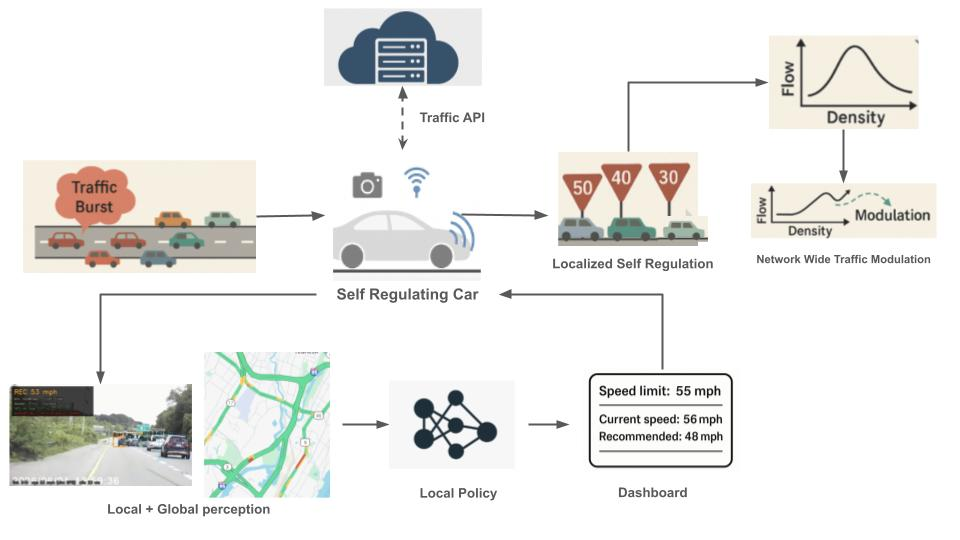
\includegraphics[width=\linewidth]{images/system_overview.jpg}
\caption{System overview. A burst of inflow pushes a stretch of road toward its critical density. Each equipped vehicle reads the network from a commercial probe feed (global layer) and the road ahead from its own camera (local layer), computes its advisory onboard, and shows the driver a recommended speed. The vehicles coordinate only through the feed version they read; none talks to another.}
\label{fig:overview}
\end{figure}

\noindent\textbf{Design goals.} Five requirements shape the design. The first two are derived from the jam dynamics, and the last three are to lower the adoption cost.
\begin{itemize}[wide=0pt,itemsep=1pt,topsep=2pt]
\item[(G1)] \emph{See the whole network.} A segment jams because of vehicles that entered upstream of it. Advice that prevents the jam must reach those vehicles before they arrive, so it needs the state of segments they have not yet reached.
\item[(G2)] \emph{Act before the road breaks down.} Near capacity, a jammed bottleneck serves less traffic than keeps arriving, so the jam does not drain until demand falls (Section~\ref{sec:feed}). A controller that acts only once it sees the jam must then hold traffic back for as long as demand stays high; one that acts while the road still flows can keep the jam from forming.
\item[(G3)] \emph{Give consistent advice without a coordinator or messages between vehicles.} Vehicles on the same stretch that are told different speeds drive at different speeds, which causes lane changes and braking near capacity. A central coordinator must collect every vehicle's position and stay available, and messages between vehicles need radios and a more complicated protocol. We want the effect of coordination without the required infrastructure.
\item[(G4)] \emph{Advise without touching the vehicle's controls.} Taking over the throttle or brakes requires modifying the vehicle and certifying the change for safety. The CIRCLES vehicles, for example, were modified to accept speed commands~\cite{lee2024traffic}. An advisory can be added to any car, and the driver keeps control of the vehicle.
\item[(G5)] \emph{Run on hardware a driver can buy.} The system acts only through the vehicles that carry it. The cost of equipping one vehicle therefore limits how many vehicles can take part. The rig of Section~\ref{sec:road} costs US\$500.
\end{itemize}

\begin{table}[t]
\centering
\caption{The two sources of information, as measured in this work.}
\label{tab:sources}
\footnotesize
\setlength{\tabcolsep}{4pt}
\begin{tabular}{@{}lll@{}}
\toprule
 & Feed (global layer) & Camera (local layer) \\
\midrule
Coverage & every network segment & 60\,m, own and side lanes \\
Measures & segment speed, jam factor & gaps, vehicles in range \\
Update & one version per 60\,s & every 5\,s \\
Delay to act & 99.5\,s & about 6\,s \\
Sees a jam when & speed has fallen & density is rising \\
\bottomrule
\end{tabular}
\end{table}

\noindent\textbf{One layer per source.} No single source meets G1 and G2 together (Table~\ref{tab:sources}): the feed covers the network but reports a forming jam late, and the camera reports it early but sees only the next 60\,m. The system therefore gives each source the decision it is suited to. The global layer sets a plan for the whole network from the feed, and the local layer may lower one vehicle's speed below that plan when its own camera sees the road filling. A safety filter follows both: it raises an advisory far below the surrounding traffic, since a much slower vehicle is itself an obstruction, and withholds it when the gap ahead, or the time to close it, falls below a minimum.

\noindent\textbf{Inputs and outputs.} The network is divided into super-segments, twelve on the network we evaluate. For each, the global layer reads three fields from the HERE Traffic API~\cite{here_traffic_api}, \texttt{speed}, \texttt{free\_flow} and \texttt{jam\_factor}, and two from the map, lane count and length. HERE does not publish how it computes the jam factor, so from the patent that defines it by travel time relative to free-flow travel time~\cite{auxer2007rating} we use a simple model, $10(1-v/v_f)$ clipped to $[0,10]$, for speed $v$ and free-flow speed $v_f$. The output for each super-segment is one of three fractions, 0.5, 0.75 or 1.0, of its static speed limit; we scale the static limit rather than the feed's free-flow reading so that a live reading does not enter the loop as both observation and base.
